
  Using these inequalities, we now construct another approximation of consumption function, $\tilde{\cFunc}_{t}({m}_{t})$, whose performance is better for points lying outside the original grid. Denote the largest and smallest points on that grid by $\bar{m}$ and $\underaccent{\bar}{m}$ respectively.  The above inequality then tells us that we have a limiting function $ \bar{\cFunc}_{t}(\ushort{m}_{t}+\aboveMin \mNrm_{t})$ for values of m, greater than $\bar{m}$, i.e., for values of $m_t > \bar{m} $  and $m_t \rightarrow \infty $, the behavior of $\tilde{\cFunc}_{t}({m}_{t})$ is anchored by $ \bar{\cFunc}_{t}({m}_{t})$. More precisely, our improved consumption function's behavior would be governed by following  rules:
\begin{itemize}
\item $\tilde{\cFunc}_{t}({m}_{t})$  = $ \cFunc_{t}({m}_{t})$ when $m_t$ falls inside the specified grid, i.e.\ when $m_t$ < $\bar{m}$
\item $\tilde{\cFunc}_{t}({m}_{t})  \rightarrow    \cFuncBelow_{t}(m_{t})  $  as $m_t \rightarrow 0$.
\item $\tilde{\cFunc}_{t}({m}_{t})  \rightarrow   \bar{\cFunc}_{t}({m}_{t}) $  as $m_t \rightarrow \infty$.
\end{itemize}

With the above principle in mind, start with a point $m$ beyond the specified grid, $m > \bar{m}$. Since the gridpoints in our case are one-dimensional, the point in the grid closest to $m$ is $\bar{m}$. This method first calculates a standardized distance between $m$ and $\bar{m}$ as:
\begin{align*}
  d(m, \bar{m}) & =  \left| \frac{m - \bar{m}}{\bar{m}} \right|
\end{align*}
and uses it to compute the combination between extrapolated value  $ \cFunc_{t}({m}_{t})$ and the limit-value $\bar{\cFunc}_{t}({m}_{t}) $ as :

\[  \tilde{\cFunc}_{t}({m}_{t}) = e^{-d(m, \bar{m})} \times   \cFunc_{t}({m}_{t})  +  (1-e^{-d(m, \bar{m})})\times  \bar{\cFunc}_{t}({m}_{t})\]

i.e. our improved approximation of consumption function is a weighted average of  $ \cFunc_{t}({m}_{t})$ and  $\bar{\cFunc}_{t}({m}_{t}) $. As the distance between $m$ and $\bar{m}$ grows,  $\bar{\cFunc}_{t}({m}_{t})$ is given more weight. That makes intuitive sense as $m$ being far outside the pre-specified grid point range corresponds to the case of a large realization of temporary shock. And that means, consumer would have enormous market resources at its disposal than usual, in which case its consumption behavior would closely follow that of an optimist (i.e. $\bar{\cFunc}_{t}({m}_{t})$).
Readers interested in alternative methods of extrapolation should refer this HARK \href{https://github.com/econ-ark/HARK/blob/master/examples/Interpolation/DecayInterp.ipynb}{documentation}.

So far, we have discussed the procedure to carry out extrapolation when the point is larger than the maximum grid point that was specified with $\bar{\cFunc}(m)$ as the benchmark function. By similar reasoning, we can also conduct extrapolation when the point is smaller than the minimum grid point with  $\cFuncBelow(m)$ serving now as the benchmark function anchoring the behavior of approximate consumption function in that point range.


  Because this method relies upon the fact that the problem is easy to
  solve if the decision maker has unreasonable views (either in the
  optimistic or the pessimistic direction), and because the correct
  solution is always between these immoderate extremes, we call our
  solution procedure the `method of moderation.'

  Results are shown in Figure~\ref{fig:ExtrapProblemSolved}; a reader
  with very good eyesight might be able to detect the barest hint of a
  discrepancy between the Truth and the Approximation at the far
  righthand edge of the figure\ctw{.}{ -- a stark contrast with the calamitous
    divergence evident in Figure~\ref{fig:ExtrapProblem}.}{}
  \hypertarget{ExtrapProblemSolvedPlot}{}
  \begin{figure}
    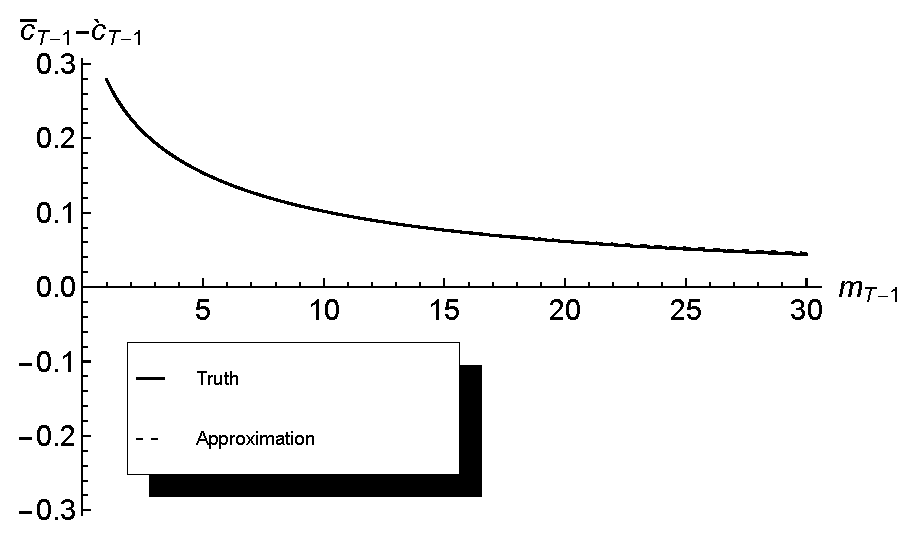
\includegraphics{./Figures/ExtrapProblemSolvedPlot}
    \caption{Extrapolated $\Alt{\Hi{\cFunc}}_{T-1}$ Constructed Using the Method of Moderation}
    \label{fig:ExtrapProblemSolved}
  \end{figure}

